\documentclass[11pt]{article}

% Change "review" to "final" to generate the final (sometimes called camera-ready) version.
% Change to "preprint" to generate a non-anonymous version with page numbers.
\usepackage[review]{acl}

% Standard package includes
\usepackage{times}
\usepackage{latexsym}

% For proper rendering and hyphenation of words containing Latin characters (including in bib files)
\usepackage[T1]{fontenc}

% This assumes your files are encoded as UTF8
\usepackage[utf8]{inputenc}

\usepackage{microtype}
\usepackage{graphicx}
\usepackage{booktabs}
\usepackage{tabularx}
\usepackage{xcolor}
\usepackage{hyperref}

\definecolor{primary}{RGB}{30, 41, 59}
\definecolor{secondary}{RGB}{71, 85, 105}
\definecolor{accent}{RGB}{2, 132, 199}

\hypersetup{colorlinks=true, linkcolor=accent, urlcolor=accent}

\title{Instructions for *ACL Proceedings}

\author{First Author \\ Affiliation / Address line 1 \\ Affiliation / Address
line 2 \\ Affiliation / Address line 3 \\ \texttt{email@domain} \\\And Second
Author \\ Affiliation / Address line 1 \\ Affiliation / Address line 2 \\
Affiliation / Address line 3 \\ \texttt{email@domain} \\}

\begin{document}
    \maketitle
    \begin{abstract}
        foundational algorithms~\citep{Aho:72}. This is a placeholder
    \end{abstract}

    \section{Introduction}

    \section{Results}
    \begin{table}[htbp]
        \centering
        \vspace{0.5em}
        \small
        \begin{tabular}{lccc}
            \toprule \textbf{Language} & \textbf{DeBERTa} & \textbf{Qwen} & \textbf{XLM-RoBERTa} \\
            \midrule Acholi            & 0.1994           & 0.0989        & 0.0438               \\
            Luganda                    & 0.1933           & 0.1253        & 0.0853               \\
            Masaaba                    & 0.1800           & 0.0817        & 0.0814               \\
            Nyankole                   & 0.1924           & 0.1210        & 0.0865               \\
            Soga                       & 0.1911           & 0.1170        & 0.0946               \\
            Akan                       & 0.1891           & 0.1277        & 0.0651               \\
            Ewe                        & 0.1813           & 0.0633        & 0.0527               \\
            Dagbani                    & 0.2281           & 0.0730        & 0.0509               \\
            Norwegian                  & 0.1251           & 0.0663        & 0.0744               \\
            Slovak                     & 0.1232           & 0.0656        & 0.0751               \\
            Serbian                    & 0.1313           & 0.1568        & 0.1456               \\
            Bulgarian                  & 0.1145           & 0.0710        & 0.0636               \\
            Czech                      & 0.1216           & 0.0634        & 0.0741               \\
            Turkish                    & 0.1389           & 0.0700        & 0.0819               \\
            Persian                    & 0.1374           & 0.0818        & 0.0657               \\
            Vietnamese                 & 0.1361           & 0.0614        & 0.0720               \\
            Indonesian                 & 0.0958           & 0.0566        & 0.0727               \\
            Assamese                   & 0.1815           & 0.0419        & 0.0648               \\
            Dogri                      & 0.1576           & 0.0957        & 0.0506               \\
            GOM                        & 0.1757           & 0.0730        & 0.0554               \\
            Kannada                    & 0.1461           & 0.0429        & 0.1174               \\
            Nepali                     & 0.1900           & 0.0551        & 0.0296               \\
            Tamil                      & 0.1330           & 0.0468        & 0.0689               \\
            Sindhi                     & 0.1466           & 0.0534        & 0.0461               \\
            \bottomrule
        \end{tabular}
        \caption{Silhouette Scores per Language Across Models}
        \label{tab:silhouette_scores}
    \end{table}

    % Using table* to span both columns for wide/long tables
    \begin{table*}
        [htbp]
        \centering
        \small
        \begin{tabular}{llcc}
            \toprule \textbf{Language 1} & \textbf{Language 2} & \textbf{Matrix Shape} & \textbf{Mean Cosine Sim.} \\
            \midrule Acholi              & Luganda             & (4108, 5455)          & 0.9508                    \\
            Acholi                       & Masaaba             & (4108, 6867)          & 0.9619                    \\
            Acholi                       & Nyankole            & (4108, 6783)          & 0.9583                    \\
            Acholi                       & Soga                & (4108, 6219)          & 0.9615                    \\
            Acholi                       & Akan                & (4108, 10107)         & 0.9490                    \\
            Acholi                       & Ewe                 & (4108, 15054)         & 0.9513                    \\
            Acholi                       & Dagbani             & (4108, 14231)         & 0.9727                    \\
            Acholi                       & Norwegian           & (4108, 534)           & 0.6627                    \\
            Acholi                       & Slovak              & (4108, 538)           & 0.6109                    \\
            Acholi                       & Serbian             & (4108, 546)           & 0.6337                    \\
            Acholi                       & Bulgarian           & (4108, 539)           & 0.5994                    \\
            Acholi                       & Czech               & (4108, 529)           & 0.5950                    \\
            Acholi                       & Turkish             & (4108, 535)           & 0.6592                    \\
            Acholi                       & Persian             & (4108, 535)           & 0.7178                    \\
            Acholi                       & Vietnamese          & (4108, 530)           & 0.4640                    \\
            Acholi                       & Indonesian          & (4108, 548)           & 0.6435                    \\
            Acholi                       & Assamese            & (4108, 4829)          & 0.7712                    \\
            Acholi                       & Dogri               & (4108, 4874)          & 0.8890                    \\
            Acholi                       & GOM                 & (4108, 4831)          & 0.9279                    \\
            Acholi                       & Kannada             & (4108, 11643)         & 0.7280                    \\
            Acholi                       & Nepali              & (4108, 4814)          & 0.7242                    \\
            Acholi                       & Tamil               & (4108, 12841)         & 0.7609                    \\
            Acholi                       & Sindhi              & (4108, 4831)          & 0.7811                    \\
            Luganda                      & Nyankole            & (5455, 6783)          & 0.9677                    \\
            Luganda                      & Soga                & (5455, 6219)          & 0.9679                    \\
            Norwegian                    & Slovak              & (534, 538)            & 0.9842                    \\
            Norwegian                    & Serbian             & (534, 546)            & 0.9835                    \\
            Slovak                       & Czech               & (538, 529)            & 0.9935                    \\
            Kannada                      & Nepali              & (11643, 4814)         & 0.9748                    \\
            Nepali                       & Sindhi              & (4814, 4831)          & 0.9694                    \\
            \bottomrule
        \end{tabular}
        \caption{Cross-Lingual Cosine Similarity Metrics (DeBERTa Model)}
        \label{tab:deberta_sim}
    \end{table*}

    \begin{table*}
        [htbp]
        \centering
        \small
        \begin{tabular}{llcc}
            \toprule \textbf{Language 1} & \textbf{Language 2} & \textbf{Matrix Shape} & \textbf{Mean Cosine Sim.} \\
            \midrule Acholi              & Luganda             & (4108, 5455)          & 0.9033                    \\
            Acholi                       & Masaaba             & (4108, 6867)          & 0.8999                    \\
            Acholi                       & Nyankole            & (4108, 6783)          & 0.9018                    \\
            Acholi                       & Soga                & (4108, 6219)          & 0.9156                    \\
            Acholi                       & Akan                & (4108, 10107)         & 0.8560                    \\
            Acholi                       & Norwegian           & (4108, 534)           & 0.5413                    \\
            Acholi                       & Bulgarian           & (4108, 539)           & -0.1191                   \\
            Acholi                       & Persian             & (4108, 535)           & -0.1207                   \\
            Acholi                       & Kannada             & (4108, 11643)         & -0.0689                   \\
            Luganda                      & Nyankole            & (5455, 6783)          & 0.9606                    \\
            Norwegian                    & Slovak              & (534, 538)            & 0.4964                    \\
            Slovak                       & Czech               & (538, 529)            & 0.8998                    \\
            Dogri                        & GOM                 & (4874, 4831)          & 0.9543                    \\
            Kannada                      & Tamil               & (11643, 12841)        & 0.5917                    \\
            \bottomrule
        \end{tabular}
        \caption{Cross-Lingual Cosine Similarity Metrics (Qwen Model)}
        \label{tab:qwen_sim}
    \end{table*}

    \begin{table*}
        [htbp]
        \centering
        \small
        \begin{tabular}{llcc}
            \toprule \textbf{Language 1} & \textbf{Language 2} & \textbf{Matrix Shape} & \textbf{Mean Cosine Sim.} \\
            \midrule Acholi              & Luganda             & (4108, 5455)          & 0.9965                    \\
            Acholi                       & Masaaba             & (4108, 6867)          & 0.9962                    \\
            Acholi                       & Nyankole            & (4108, 6783)          & 0.9967                    \\
            Acholi                       & Norwegian           & (4108, 534)           & 0.9894                    \\
            Luganda                      & Nyankole            & (5455, 6783)          & 0.9971                    \\
            Norwegian                    & Slovak              & (534, 538)            & 0.9974                    \\
            Slovak                       & Czech               & (538, 529)            & 0.9987                    \\
            Vietnamese                   & Indonesian          & (530, 548)            & 0.9983                    \\
            Dogri                        & GOM                 & (4874, 4831)          & 0.9980                    \\
            Kannada                      & Tamil               & (11643, 12841)        & 0.9975                    \\
            \bottomrule
        \end{tabular}
        \caption{Cross-Lingual Cosine Similarity Metrics (XLM-RoBERTa Model)}
        \label{tab:xlmr_sim}
    \end{table*}

    \begin{figure*}[t]
        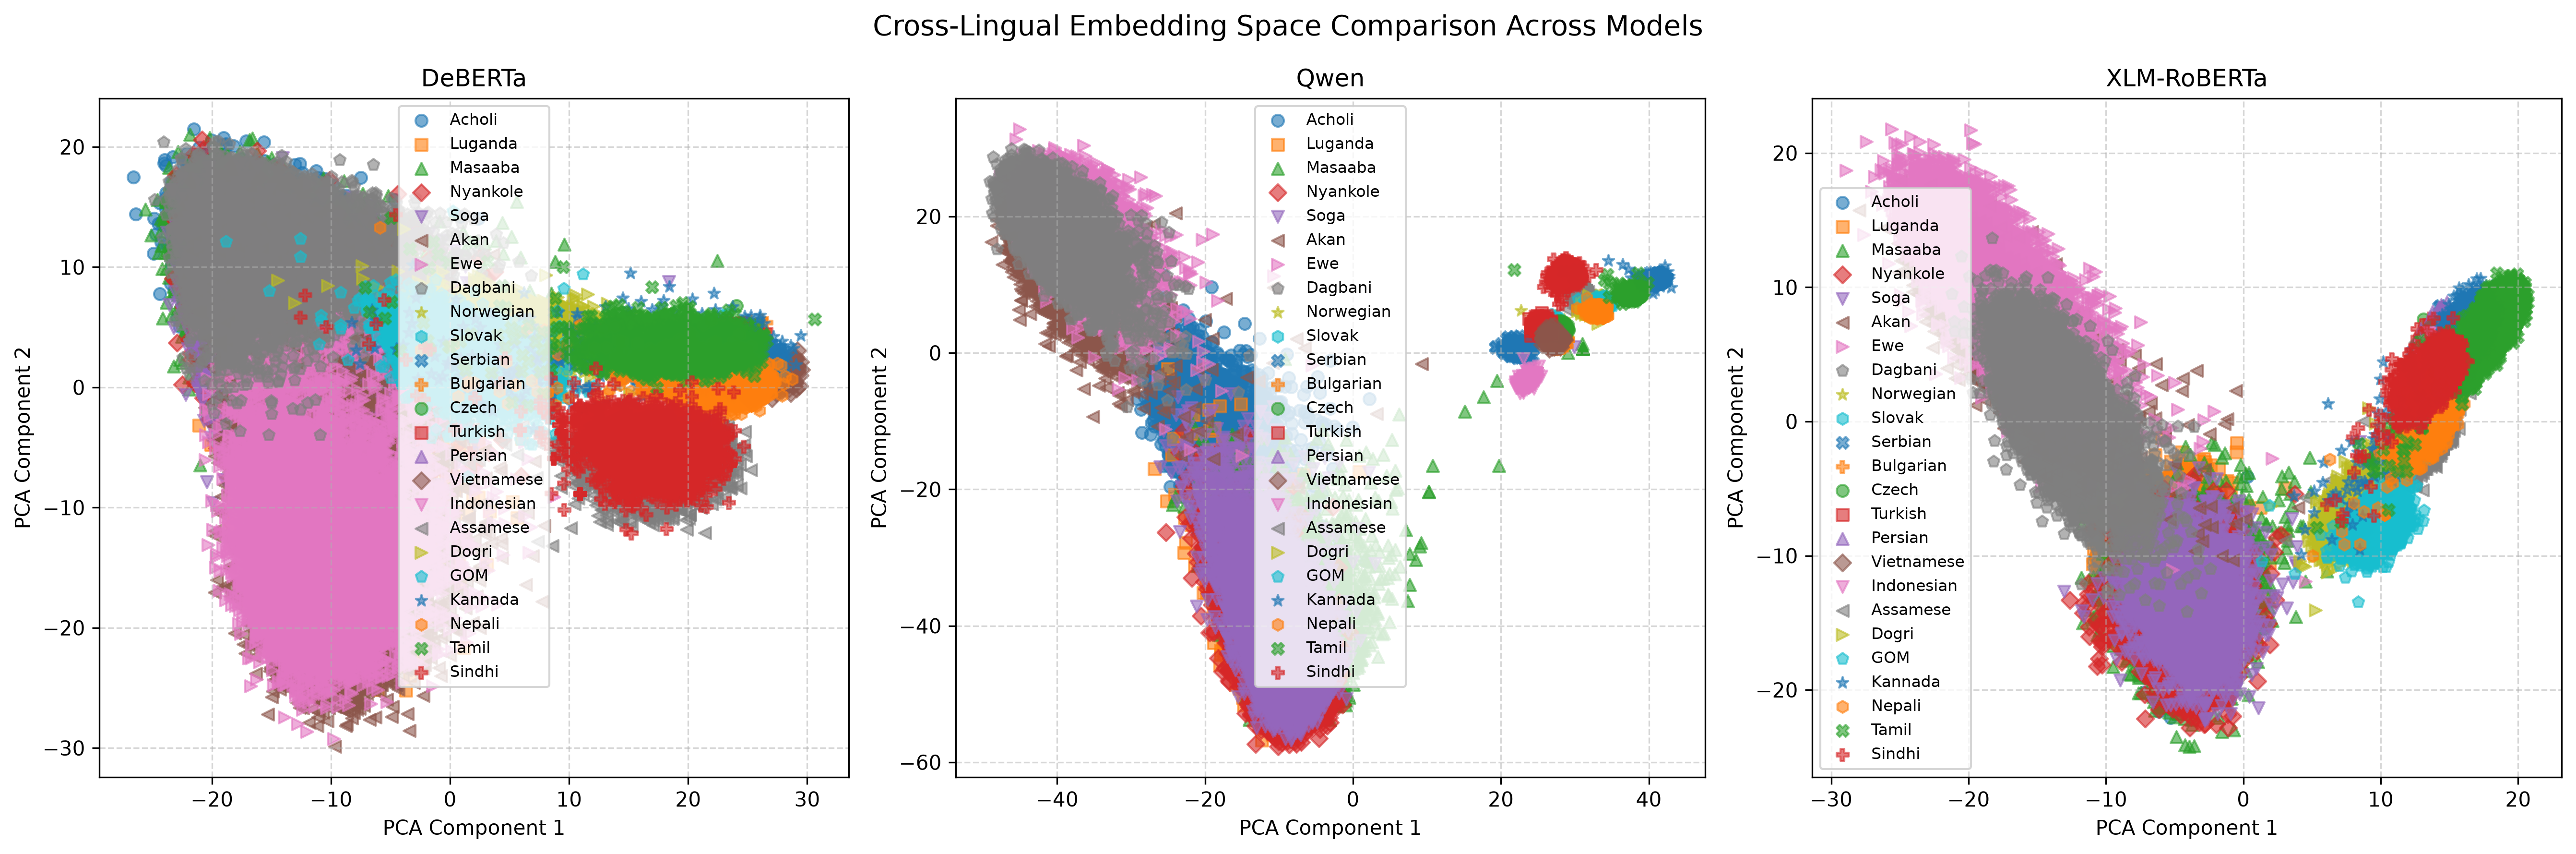
\includegraphics[width=\linewidth]{
            multilingual_models_embedding_space.png
        }
        \caption{A minimal working example to demonstrate how to place two
        images side-by-side.}
    \end{figure*}

    \bibliography{custom}

    \appendix
\end{document}